% DRAFT written by Claude Code for the author to review. Every number comes from a file in results/ or configs/ (named in a % comment).
% Red [TODO(verify): ...] marks facts that are not in the repo. Red [PLACEHOLDER: ...] marks author/link fields.
\documentclass[conference]{IEEEtran}
\IEEEoverridecommandlockouts
\usepackage{cite}
\usepackage{amsmath,amssymb,amsfonts}
\usepackage{graphicx}
\usepackage{textcomp}
\usepackage{xcolor}
\usepackage{booktabs}
\usepackage{url}
\usepackage[hidelinks]{hyperref}
\def\BibTeX{{\rm B\kern-.05em{\sc i\kern-.025em b}\kern-.08em
    T\kern-.1667em\lower.7ex\hbox{E}\kern-.125emX}}

\newcommand{\todo}[1]{\textcolor{red}{[TODO(verify): #1]}}
\newcommand{\placeholder}[1]{\textcolor{red}{[PLACEHOLDER: #1]}}
\newcommand{\code}[1]{\texttt{#1}}

\begin{document}

\title{TrialMatch Transformer: Fine-Tuning, KV-Cache, Tiled Attention and Speculative Decoding for Clinical-Trial Criterion Screening}

\author{\IEEEauthorblockN{\placeholder{author name}}
\IEEEauthorblockA{\placeholder{affiliation, city, country}\\
\placeholder{email}}
\and
\IEEEauthorblockN{Links}
\IEEEauthorblockA{Code: \placeholder{GitHub URL}\\
Weights: \placeholder{Hugging Face Hub model id}\\
Video: \placeholder{video link}}
}

\maketitle

\begin{abstract}
We build an educational system that reads a short patient note and one inclusion or exclusion criterion of a clinical trial and returns a criterion-level label with the numbers of the supporting note sentences. We fine-tune Qwen3-4B with QLoRA on the TrialGPT criterion annotations using a patient-grouped split of 37/8/8 patients. On the held-out test split (206 criterion rows, 8 patients, evaluated once) the fine-tuned model reaches accuracy 0.767 and macro-F1 0.726 over the classes present, against 0.665 and 0.523 for the base model and 0.626 and 0.272 for a majority-label baseline. The dominant error is answering ``not excluded'' where annotators judged ``not enough information''. We also implement a KV-cache decoder, an online-softmax tiled attention and greedy speculative decoding from scratch and measure them on a Tesla T4. The cache gives a 3.0 times speed-up on real validation prompts and up to 7.1 times at 1024 input tokens; tiled attention uses up to 180 times less peak memory than the reference at 4096 tokens; speculative decoding with an untuned Qwen3-0.6B draft gave no speed-up on real validation prompts. This is an educational prototype, not a clinical enrollment tool.
\end{abstract}

\begin{IEEEkeywords}
clinical trial matching, LoRA, KV cache, attention, speculative decoding
\end{IEEEkeywords}

\section{Introduction}
Matching a patient to a clinical trial means checking the patient against many inclusion and exclusion criteria. A useful assistant would, for each criterion, say whether the patient meets it and point to the note sentences that justify the answer. We study a small version of this problem with an open model that fits on a free Colab T4 GPU, and we use the project to implement and measure three inference techniques by hand: a key/value (KV) cache, a tiled attention with online softmax, and speculative decoding.

Contributions: (i) a leakage-controlled data pipeline with a strict JSON output format, a parser and metrics that treat invalid outputs and empty evidence explicitly; (ii) a QLoRA fine-tuned Qwen3-4B evaluated on validation and, once, on test; (iii) tested hand-written cached decoding, tiled attention and speculative decoding, benchmarked on a T4, including a documented case of fp16 near-tie mismatches; (iv) a browser application whose demo mode never presents invented output as a model prediction. The system is an educational prototype and must not be used for real patient care or trial enrollment.

\section{Related Work}
\emph{Trial matching.} The data are the criterion-level annotations released with TrialGPT \cite{trialgpt}, in which a large language model judges each criterion and cites note sentences. The release also contains GPT-4 predictions, which we treat as forbidden inputs (Section~\ref{sec:data}). \todo{check the TrialGPT claims against the paper}

\emph{Models and fine-tuning.} We use Qwen3 \cite{qwen3}, LoRA adapters \cite{lora} and 4-bit base weights as in QLoRA \cite{qlora}.

\emph{Efficient inference.} Attention follows \cite{vaswani}; the online softmax \cite{milakov} and its blockwise use in FlashAttention \cite{flashattention} motivate our tiled version, which is plain PyTorch and therefore not fused. Grouped-query attention \cite{gqa} and rotary embeddings \cite{rope} determine the size and indexing of the KV cache. Speculative decoding \cite{leviathan,chen2023} motivates our greedy draft-and-verify decoder. All references in this draft are marked VERIFY in the bibliography file because they could not be checked.

\section{Data and Task}\label{sec:data}
The annotation set has 1,015 criterion rows from 53 patients and 103 trials, with 5 to 43 rows per patient and exactly one note per patient (6.2 sentences on average, 3 to 14). % results/metrics/data_inspection.json, docs/data_inspection.md
There are 659 exclusion and 356 inclusion rows. Labels are kept as annotated: inclusion criteria use \emph{included, not included, not enough information (NEI), not applicable}; exclusion criteria use \emph{excluded, not excluded, NEI, not applicable}. The gold label is the expert label and the gold evidence the expert sentence list.

\emph{Leakage control.} Four columns hold previous model outputs (\code{gpt4\_explanation}, \code{explanation\_correctness}, \code{gpt4\_sentences}, \code{gpt4\_eligibility}) and are removed from the processed files. The \code{training} column has unknown meaning and varies within 44 of 53 patients, so it is unused. % docs/decisions.md 2026-11-06
Rows follow their patient: sorted patient ids are shuffled with seed 42 and the first 37, next 8 and last 8 patients form train, validation and test (603, 206, 206 rows). % docs/label_distribution.md, docs/decisions.md
One row with a null criterion text (annotation 883, in train) is skipped.

\begin{table}[t]
\caption{Gold label counts (rows) per split. Source: \protect\path{docs/label_distribution.md}.}\label{tab:labels}
\centering\small\setlength{\tabcolsep}{4pt}
\begin{tabular}{lrrrr}
\toprule
 & train & val & test & all\\
\midrule
rows & 603 & 206 & 206 & 1015\\
incl.: included & 88 & 35 & 27 & 150\\
incl.: not included & 13 & 3 & 7 & 23\\
incl.: NEI & 109 & 27 & 38 & 174\\
incl.: not applicable & 5 & 1 & 3 & 9\\
excl.: excluded & 8 & 2 & 0 & 10\\
excl.: not excluded & 292 & 101 & 91 & 484\\
excl.: NEI & 65 & 26 & 28 & 119\\
excl.: not applicable & 23 & 11 & 12 & 46\\
\bottomrule
\end{tabular}
\end{table}

Table~\ref{tab:labels} shows the main difficulty: the labels are very imbalanced. ``Not excluded'' alone is 484 of 659 exclusion rows (73.4\%), ``excluded'' has 10 rows overall and \emph{none} in test, and inclusion ``not applicable'' has 9 rows. About 60\% of rows have empty gold evidence (0.601 in \path{docs/data_inspection.md}), so an empty evidence list is a valid and very common answer and is scored as such.

\emph{Prompt and output.} The model sees only the numbered note sentences, the criterion type and the criterion text, and answers with a JSON object \code{\{"label": ..., "evidence\_ids": [...]\}} with ascending unique integer ids. No explanation is generated, because no gold explanations exist and the GPT-4 ones are forbidden. The parser never maps an invalid output to a valid label. % README.md (src/trialmatch/model/*)
The longest prompt plus target is 618 tokens with the Qwen chat template, so a maximum length of 768 truncates nothing. % results/metrics/token_stats.json, configs/train.yaml

\section{Methods}
\subsection{Fine-tuning}
We fine-tune Qwen3-4B (4.02 B parameters, 36 layers, 32 query and 8 key/value heads) % docs/model_facts.md
with QLoRA: NF4 4-bit base weights, fp16 compute, LoRA rank 16, alpha 32, dropout 0.05 on the attention and MLP projections only (embeddings are tied to the output layer, so \code{lm\_head} is not adapted). Learning rate $2\times10^{-4}$, cosine schedule, 5\% warm-up, 3 epochs, per-device batch 4 with 4 accumulation steps (effective batch 16), gradient checkpointing, seed 42. % configs/train.yaml
The loss covers the answer JSON and the end token only. Qwen3-0.6B is the speculative draft; Qwen3-1.7B was defined as a fallback but never trained. % docs/decisions.md 2026-11-07

\subsection{Evaluation protocol and metrics}
All systems use greedy decoding with at most 64 new tokens and the same prompt. % configs/train.yaml
Accuracy counts every row; an invalid output is a separate, always-wrong prediction. Macro-F1 is reported over the classes present in the gold labels and over the full label set; they differ when a class has no gold rows. Evidence is scored per row as a set of sentence ids: both empty scores 1, exactly one empty scores 0; micro-F1 pools sentence counts, macro-F1 averages rows; each is reported including and excluding rows with empty gold evidence. The baseline predicts the training-majority label per criterion type and always-empty evidence. % docs/decisions.md 2026-11-07
The test split needs an explicit confirmation flag and a single run; it was evaluated once with the merged model. % docs/decisions.md 2026-11-07, results/eval/test_split_evaluated.json

\subsection{Merged fp16 model}
The adapter was trained on a 4-bit base. For all inference benchmarks we merge it into fp16 weights (\code{merge\_and\_unload}), giving one model of 4,022,468,096 parameters. % results/logs/merge_verify.json, results/benchmarks/kv_cache_20261107_192136.json
On four validation prompts the merged and unmerged logits differ by at most 0.048 and the top-1 token agrees on all four. % results/logs/merge_verify.json

\subsection{Manual KV-cache decoder}
\code{cached\_greedy\_decode} (\path{src/trialmatch/inference/kv_cache/cached_decode.py}) prefills the prompt once, keeps \code{past\_key\_values} itself, then feeds only the newest token with explicit \code{position\_ids} (tokens so far), \code{cache\_position} and a 2-D mask that grows by one column per step, asserting that the cache grows by exactly one position. \code{reference\_greedy\_decode} re-runs the full forward at every step. Both use argmax.

\subsection{Tiled attention}
\code{tiled\_attention} processes keys in blocks and keeps a running maximum $m$, normaliser $l$ and output $o$; on a new block it rescales by $\alpha=\exp(m-m_{\mathrm{new}})$, so $o/l$ is softmax attention over the keys seen so far and exact after the last block. Blocks above the causal diagonal are skipped. Query $i$ sees key $j$ iff $j\le i+(S_k-S_q)$; arithmetic is fp32 with the output cast back; grouped-query attention repeats each KV head for its query group. The reference materialises the full score matrix; torch SDPA backends are comparison only. % src/trialmatch/inference/attention/*.py

\subsection{Speculative decoding}
\code{speculative\_greedy\_decode} (batch size 1) lets the draft propose $k$ tokens, verifies them with one target forward over the last token plus the candidates, accepts the longest matching prefix, emits the target's own token as correction (or bonus when all $k$ match) and crops both caches to the accepted length. Its output equals plain greedy decoding of the target up to floating-point ties. % src/trialmatch/inference/speculative/speculative_decode.py

\subsection{Application}
A FastAPI backend with one static page offers a screening workspace (per-criterion cards with label badge, cited sentences, template explanations and a rule-based preliminary outcome stated not to be a ground-truth label) and an Inference Lab. Demo mode answers only from cached real validation predictions and otherwise says it cannot predict. % docs/decisions.md 2026-11-08, docs/app_notes.md

\section{Experimental Setup}
Training and benchmarks ran on a Colab Tesla T4 (14.56 GiB) with Python 3.13, torch 2.14.1+cu130, transformers 5.22.1, peft 0.21.2 and bitsandbytes 0.50.2. % results/logs/env_qwen3-4b_qlora_4bit.json
Training took about 33 minutes (114 optimiser steps; log from 10:40:44 to 11:13:53). % results/logs/train_qwen3-4b_qlora_4bit.jsonl
\emph{KV cache:} synthetic inputs of 128, 256, 512, 1024 tokens with 16, 64, 128 new tokens (EOS disabled) and 16 real validation prompts, 1 warm-up and 5 repeats, decoders interleaved. \emph{Attention:} random fp16 inputs, 32 query heads, 8 KV heads, head dimension 128, causal, lengths 128 to 4096, block sizes 32 to 256, 2 warm-ups, 10 repeats, error against an fp32 reference. \emph{Speculative:} untuned Qwen3-0.6B draft, $k\in\{1,2,4,8\}$, synthetic inputs of 128, 256, 512 tokens with 16/64/128 new tokens and 8 validation prompts, 3 repeats. % benchmark json args
Timings are medians unless stated; attention memory is the peak above the run's starting level.

\section{Results and Discussion}
\subsection{Classification and evidence}
\begin{table}[t]
\caption{Validation split (206 rows). Evid.\ F1 is micro-F1 over all rows (incl.) and over rows with non-empty gold evidence (excl.). Fine-tuned = 4-bit-base model. Source: \protect\path{results/metrics/val_comparison.md}.}\label{tab:val}
\centering\small\setlength{\tabcolsep}{3pt}
\begin{tabular}{lrrrrr}
\toprule
system & acc. & macro-F1 & ev.\ incl. & ev.\ excl. & invalid\\
\midrule
majority baseline & 0.621 & 0.215 & 0.000 & 0.000 & 0.000\\
base Qwen3-4B & 0.626 & 0.312 & 0.359 & 0.519 & 0.000\\
fine-tuned & 0.748 & 0.549 & 0.529 & 0.637 & 0.000\\
\bottomrule
\end{tabular}
\end{table}

Table~\ref{tab:val} shows that the majority baseline reaches accuracy 0.621, almost the base model's 0.626, because ``not excluded'' dominates the exclusion rows; macro-F1 separates them (0.215 vs 0.312). Fine-tuning raises accuracy by 0.122 and macro-F1 by 0.237 over the base model, and evidence micro-F1 from 0.359 to 0.529. No system produced an invalid output on validation.

\begin{table}[t]
\caption{Test split (206 rows, 8 patients, one evaluation). F1 (present) / F1 (full) are macro-F1 over present and over all classes; they differ because ``excluded'' has no gold test rows. Fine-tuned = merged fp16 model. Source: \protect\path{results/metrics/test_comparison.md}.}\label{tab:test}
\centering\footnotesize\setlength{\tabcolsep}{2pt}
\begin{tabular}{lrrrrrr}
\toprule
system & acc. & F1 pres. & F1 full & ev.\ incl. & ev.\ excl. & inv.\\
\midrule
majority baseline & 0.626 & 0.272 & 0.226 & 0.000 & 0.000 & 0.000\\
base Qwen3-4B & 0.665 & 0.523 & 0.435 & 0.376 & 0.550 & 0.000\\
fine-tuned (merged) & 0.767 & 0.726 & 0.605 & 0.578 & 0.663 & 0.000\\
\bottomrule
\end{tabular}
\end{table}

On test (Table~\ref{tab:test}) the ordering is the same: accuracy 0.767 against 0.665 for the base model (+0.102) and 0.626 for the baseline; macro-F1 over present classes is 0.726 against 0.523 and 0.272. Counting the absent ``excluded'' class as F1 of 0 lowers the fine-tuned macro-F1 to 0.605, so both numbers are reported. Evidence micro-F1 rises from 0.376 to 0.578 over all rows and from 0.550 to 0.663 on rows with non-empty gold evidence. By criterion type, the fine-tuned model has accuracy 0.813 on the 75 inclusion rows and 0.740 on the 131 exclusion rows, and evidence micro-F1 over all rows of 0.676 for inclusion but only 0.314 for exclusion. % results/metrics/test_comparison.md
Validation and test use different model variants: the merged model scored 0.733 on validation against 0.748, three rows of 206. % results/eval/finetuned_merged_val_summary.json, results/eval/finetuned_val_summary.json

\begin{figure}[t]
\centering
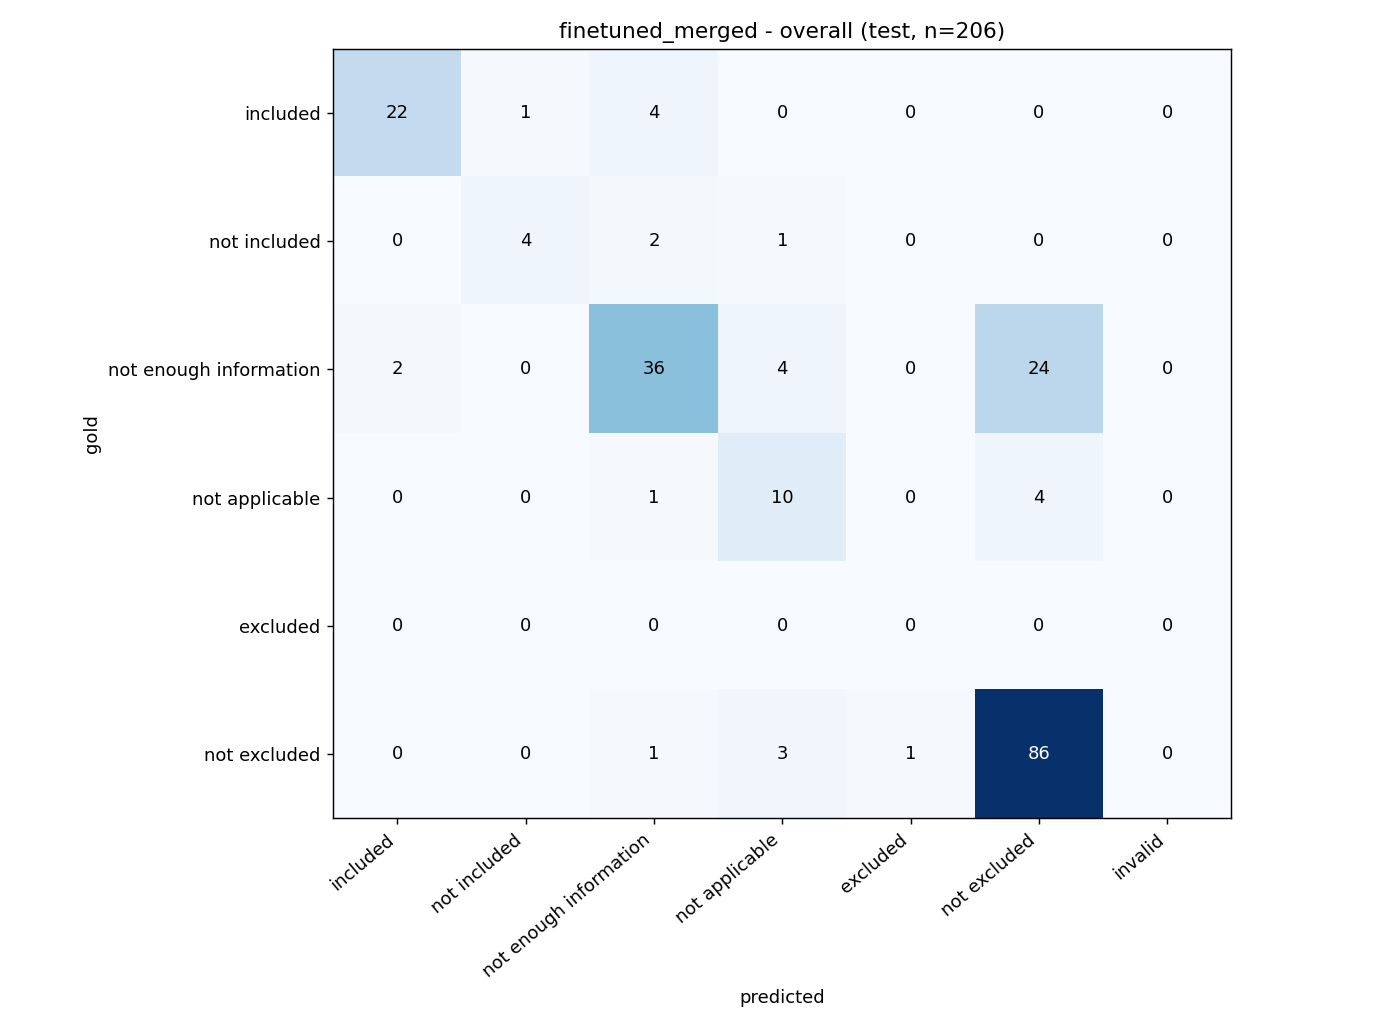
\includegraphics[width=0.95\columnwidth]{figures/confusion_finetuned_merged_overall_test.png}
\caption{Confusion matrix of the fine-tuned merged model on test (rows gold, columns predicted). Source: \protect\path{results/figures/confusion_finetuned_merged_overall_test.png}.}\label{fig:conf}
\end{figure}

Fig.~\ref{fig:conf} locates the dominant error. Of 66 gold-NEI rows (36 + 24 + 4 + 2), 36 are correct but 24 are predicted ``not excluded'' (4 ``not applicable'', 2 ``included''); in contrast 86 of 91 gold ``not excluded'' rows are correct. The per-class table agrees: NEI on exclusion criteria has precision 0.75 but recall 0.11 on test. % results/metrics/test_comparison.md; figure counts read from the image
The model seems to default to ``not excluded'' when a criterion is not discussed in the note, which is the training majority (75.3\% of train exclusion rows, \path{docs/label_distribution.md}). Of the 26 test rows with gold NEI and a decided prediction, 18 come from one patient, who accounts for 25 of the 81 test errors. % results/error_analysis/test_finetuned_merged_errors.csv
Drafted error cases are in \path{docs/error_analysis.md}: polarity errors on the rare ``excluded'' class, over-citation of the whole note, and citation of the boilerplate consent sentence (4 validation rows, 1 test row). The causes given there are hypotheses (``likely'') because we cannot inspect the model.

\begin{figure}[t]
\centering
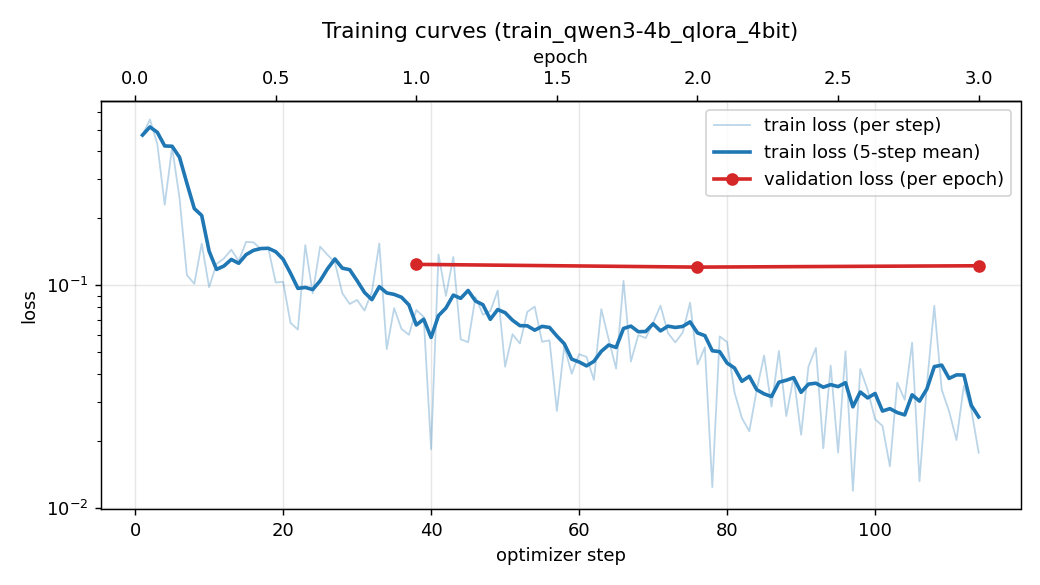
\includegraphics[width=\columnwidth]{figures/training_curves.png}
\caption{Training and validation loss. Source: \protect\path{results/figures/training_curves.png}.}\label{fig:train}
\end{figure}

Fig.~\ref{fig:train} shows the training loss falling from 0.473 at step 1 to 0.018 at step 114 while the validation loss stays near 0.12 (0.124, 0.121, 0.123 after epochs 1 to 3). A flat validation loss with a falling training loss is consistent with overfitting a 603-row training set; we ran no ablation (fewer epochs, other ranks) to confirm this. % results/logs/train_qwen3-4b_qlora_4bit.jsonl

\subsection{KV cache}
\begin{table}[t]
\caption{Cached vs.\ uncached greedy decoding on the T4: median total time (s) and speed-up (our division of medians). Source: \protect\path{results/benchmarks/kv_cache_20261107_192136.json}.}\label{tab:kv}
\centering\small\setlength{\tabcolsep}{3pt}
\begin{tabular}{rrrrr}
\toprule
input & new & cached & uncached & speed-up\\
\midrule
128 & 16 & 1.573 & 1.470 & 0.93\\
128 & 128 & 11.649 & 16.646 & 1.43\\
256 & 128 & 11.305 & 25.972 & 2.30\\
512 & 128 & 10.125 & 42.983 & 4.25\\
1024 & 16 & 1.680 & 9.745 & 5.80\\
1024 & 128 & 11.420 & 81.125 & 7.10\\
val (16) & 15--38 & 1.219 & 3.025 & 3.02\\
\bottomrule
\end{tabular}
\end{table}

Table~\ref{tab:kv} and Fig.~\ref{fig:kv} show that the cached decode time per token is roughly constant (78 to 96 ms at all input lengths) while the uncached decoder grows from about 93 ms per token at 128 input tokens to about 635 ms at 1024, since it reprocesses the whole sequence at each step. The speed-up therefore grows from 1.43 times at 128 input tokens to 7.10 times at 1024, and is 3.02 times (range 2.20 to 3.28) over the real validation prompts (317 to 338 input tokens). In the first row the cached decoder was not faster (0.93 times); the repeat spread (cached total standard deviation 0.187 s) exceeds that gap, so we regard it as noise. The cached decoder's peak memory above the starting level is 246.5 MiB at 1024 input tokens against 81.9 MiB uncached, on top of about 8.1 to 8.3 GB of weights; the cache itself is about 0.141 GiB at 1024 tokens by the formula. % kv_cache_20261107_192136.json, docs/memory_estimate.md

\begin{figure*}[t]
\centering
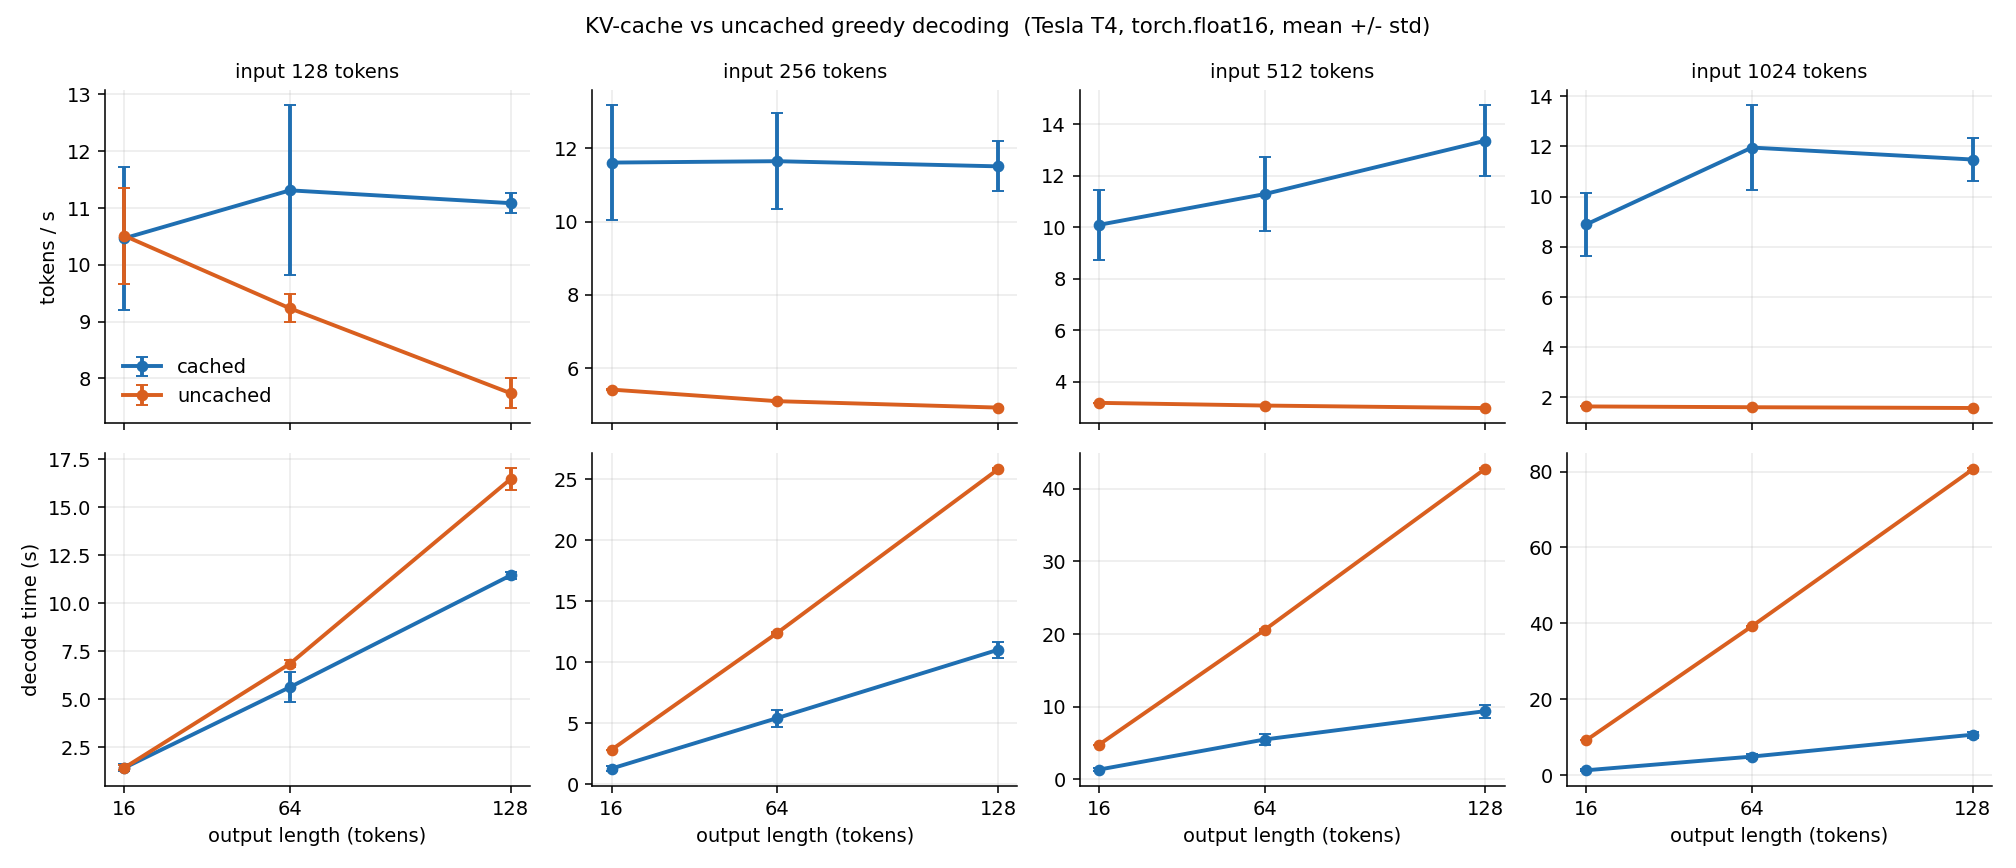
\includegraphics[width=0.95\textwidth]{figures/kv_cache.png}
\caption{Tokens per second and decode time, cached vs.\ uncached, by input length. Source: \protect\path{results/benchmarks/kv_cache_20261107_192136.png}.}\label{fig:kv}
\end{figure*}

\emph{fp16 near-tie.} One of the 12 synthetic cells (256 input, 128 new tokens) produced different tokens: the first mismatch is at step 103 with a maximum logit difference of 0.0293. All other synthetic cells and all 16 validation prompts matched. We read this as a rounding effect (prefill and single-token steps use different matrix shapes) rather than a logic error, since the same decoders agree exactly in fp32 tests on a tiny model; we did not isolate the cause, and the report does not record the top-1/top-2 margin at that step. \todo{margin at the mismatch step}

\subsection{Tiled attention}
\begin{table}[t]
\caption{Attention on the T4 (fp16, batch 1, 32 query / 8 KV heads, head dim 128): median ms / peak MiB above start. Source: \protect\path{results/benchmarks/attention_20261107_193238.json}.}\label{tab:att}
\centering\footnotesize\setlength{\tabcolsep}{2.5pt}
\begin{tabular}{rrrrr}
\toprule
seq & reference & tiled 32 & tiled 256 & SDPA eff.\\
\midrule
128 & 1.75 / 15.0 & 7.48 / 4.8 & 1.77 / 19.1 & 0.83 / 3.0\\
512 & 4.89 / 132 & 77.3 / 7.8 & 5.00 / 52.2 & 1.08 / 12.0\\
1024 & 16.9 / 457 & 309 / 11.8 & 13.6 / 56.2 & 2.23 / 24.0\\
2048 & 50.4 / 1685 & 1148 / 19.8 & 33.6 / 64.2 & 2.78 / 48.0\\
4096 & 197 / 6449 & 4515 / 35.8 & 114 / 80.2 & 8.28 / 96.0\\
\bottomrule
\end{tabular}
\end{table}

Table~\ref{tab:att} and Fig.~\ref{fig:att} show the expected memory behaviour: the reference's peak memory roughly quadruples per doubling at the long end (1684.5 to 6449.1 MiB from 2048 to 4096), whereas the tiled version stays between 35.8 and 80.2 MiB at 4096 depending on block size, 80 to 180 times smaller. The tiled results are exact to fp16 rounding: the reference, every tiled variant and the math SDPA backend share the same maximum absolute error against the fp32 reference (0.000921 at 128 tokens, 0.000966 at 4096), the memory-efficient SDPA backend has at most 0.00120, and all are within the 0.005 tolerance with no mismatch recorded. Speed is different. With block 32 the plain-PyTorch loop is 22.9 times slower than the reference at 4096 tokens (4514.71 vs 197.06 ms), and time falls about 3 to 4 times per doubling of the block size, which fits the number of Python-level iterations and kernel launches; with block 256 it is 1.7 times faster than the reference at 4096 tokens (113.85 ms) but slightly slower at short lengths (2.60 vs 2.10 ms at 256). The memory-efficient SDPA kernel is fastest everywhere (8.28 ms at 4096, 23.8 times faster than our reference); the flash backend was reported unavailable at every length (``No available kernel''), for a reason the repo does not record. \todo{why the flash SDPA backend is unavailable on this T4}
A PyTorch loop can match the memory advantage of FlashAttention-style tiling but not the speed of a fused kernel. The SDPA calls use fp16 arithmetic while ours accumulate in fp32, so the speed comparison is not like for like.

\begin{figure*}[t]
\centering
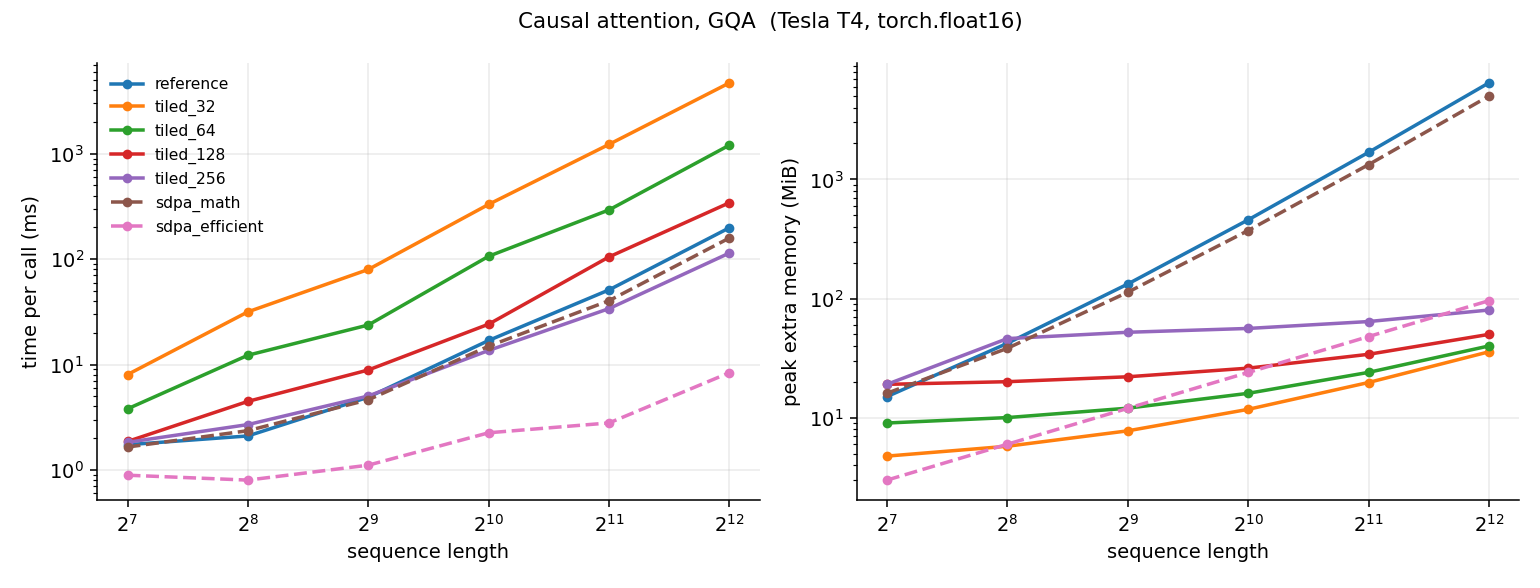
\includegraphics[width=0.85\textwidth]{figures/attention.png}
\caption{Attention time and peak extra memory vs.\ sequence length (log scale). Source: \protect\path{results/benchmarks/attention_20261107_193238.png}.}\label{fig:att}
\end{figure*}

\subsection{Speculative decoding}
\begin{table}[t]
\caption{Speculative decoding on the 8 real validation prompts (untuned Qwen3-0.6B draft): medians over prompts; speed-up = plain cached time / speculative time per prompt. Source: \protect\path{results/benchmarks/speculative_20261108_113154.json}, our medians.}\label{tab:spec}
\centering\small\setlength{\tabcolsep}{2.5pt}
\begin{tabular}{rrrrrr}
\toprule
$k$ & accept. & tok./verify & speed-up & range & draft share\\
\midrule
1 & 0.974 & 1.97 & 0.981 & 0.775--1.134 & 42.1\%\\
2 & 0.750 & 2.33 & 0.923 & 0.692--1.062 & 58.3\%\\
4 & 0.694 & 3.60 & 0.928 & 0.807--1.036 & 72.3\%\\
8 & 0.500 & 4.67 & 0.735 & 0.543--0.877 & 83.5\%\\
\bottomrule
\end{tabular}
\end{table}

Table~\ref{tab:spec} and Fig.~\ref{fig:spec} show that speculative decoding did not speed up real validation prompts. The acceptance rate falls from 0.974 at $k=1$ to 0.500 at $k=8$ and tokens per verify rise only from 1.97 to 4.67, while the draft's share of time rises from 42.1\% to 83.5\%; the median speed-up is below 1 for every $k$ (0.981, 0.923, 0.928, 0.735), and at $k=8$ no prompt was faster than plain decoding. At $k=1$ one draft step costs about 0.73 of a target verify step (0.421/0.579), far above the 0.15 parameter ratio of 0.6B to 4B; this is plausible because the draft has 28 layers against 36 and batch-size-1 decoding on a T4 is likely dominated by per-layer kernel launches. A back-of-envelope estimate of 1.97/1.73, about 1.14 times, before the extra draft prefill is consistent with the observed 0.98. \todo{profile Python overhead and the verify forward cost}
The answers are short (15 to 38 tokens): plain decoding of a validation prompt takes a median 1.037 s, 0.177 s of it prefill, leaving few iterations to amortise any overhead. On synthetic inputs the picture is similar at 128 and 256 input tokens (speed-up 0.40 to 1.145), but at 512 input tokens the acceptance rate is 1.0 for most rows and the speed-up reaches 1.288 times ($k=8$, 128 new tokens); we suspect the tiled synthetic prompt yields a repetitive continuation that the draft copies easily, but did not inspect the tokens. \todo{inspect synthetic continuations at 512 tokens}

\begin{figure*}[t]
\centering
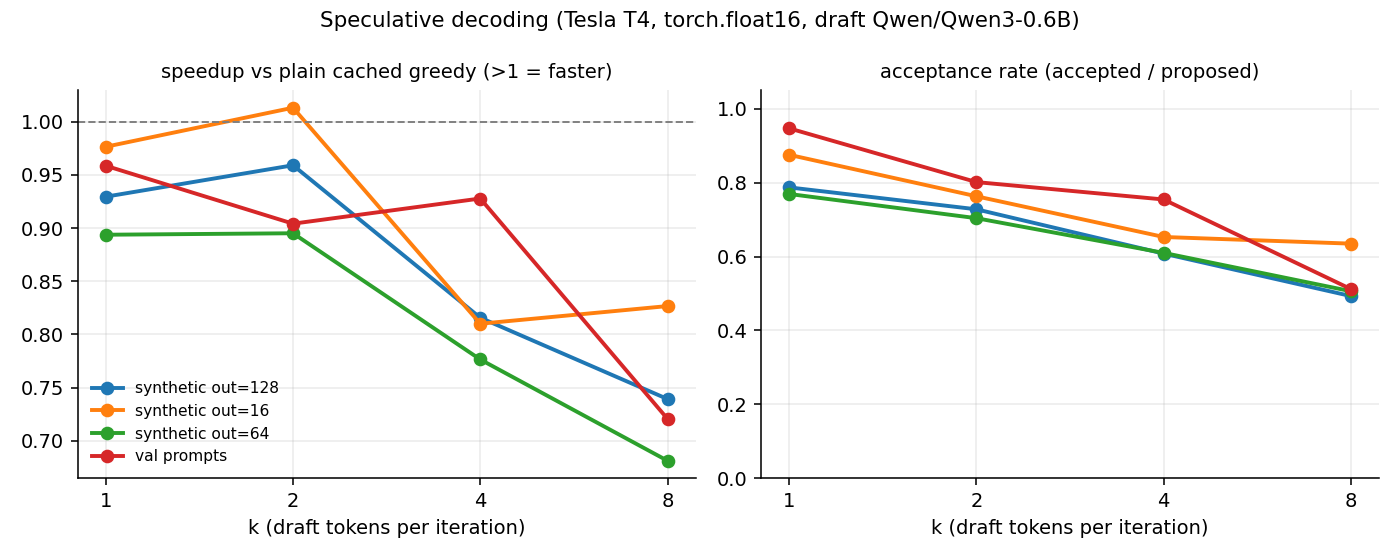
\includegraphics[width=0.85\textwidth]{figures/speculative.png}
\caption{Speed-up vs.\ plain cached greedy decoding and acceptance rate vs.\ $k$. The curves appear to be averages over input lengths while Table~\ref{tab:spec} uses medians. Source: \protect\path{results/benchmarks/speculative_20261108_113154.png}. \todo{confirm how the plot aggregates rows}}\label{fig:spec}
\end{figure*}

\emph{fp16 near-tie.} 84 of the 85 result rows produce the same tokens as plain decoding. The exception (256 input tokens, 128 new tokens, $k=1$) first differs at step 64 with a maximum logit gap of 0.0234 and a plain top-1/top-2 margin of exactly 0.0: the two best logits were tied in fp16 and the chosen token depends on rounding. We read this as a tie, consistent with the 84 identical rows, but did not isolate the cause.

\section{Limitations}
\begin{itemize}
\item \textbf{Single seed, single run.} One training run (seed 42) and one setting; no confidence intervals. \todo{any other training run outside the repo}
\item \textbf{Small test set.} 8 patients and 206 rows; differences of a few rows are within noise, and rows of one patient are correlated.
\item \textbf{No ``excluded'' rows in test.} The class has zero support on test and only 2 rows on validation.
\item \textbf{Merged vs.\ 4-bit model.} Validation used the 4-bit-base model (0.748); test and benchmarks used the merged fp16 model (0.733 on validation).
\item \textbf{CPU vs.\ T4.} All timings are from one Colab T4. The app was tested on CPU with fake or tiny models; the real 4B model on CPU and the UI in a real browser were not exercised by the assistant, and the README's CPU time per criterion (1 to 3 minutes) is a reasoned estimate. CPU numerics can differ from T4 fp16.
\item \textbf{fp16 near-ties.} One KV-cache cell (step 103, logit gap 0.0293) and one speculative row (step 64, margin 0.0) differ from the reference.
\item \textbf{Evidence weaknesses.} Exclusion evidence micro-F1 is 0.314 on test; the model over-cites, under-cites and sometimes cites the consent sentence. About 60\% of gold evidence lists are empty, which inflates metrics that include them; both views are reported.
\item \textbf{Educational implementations.} Speculative decoding is batch size 1 with an untuned draft and gave no speed-up on real prompts; tiled attention is plain PyTorch, not used inside the model, and slower than fused kernels.
\item \textbf{Educational prototype.} The preliminary outcome is a rule over criterion labels, not validated against patient-level verdicts; the system must not be used for clinical decisions.
\item \textbf{Unrecorded app observations.} A myocardial infarction three months ago labelled ``not excluded'' for a six-month exclusion, and a never-mentioned criterion labelled ``not excluded'', were observed in the app but are not saved in the repo. \todo{attach saved report or screenshot}
\end{itemize}

\section{Conclusion}
QLoRA fine-tuning of Qwen3-4B on 603 patient-grouped rows improves criterion-level accuracy from 0.665 to 0.767 and macro-F1 over present classes from 0.523 to 0.726 on a held-out test split, and improves evidence F1, but the model tends to answer ``not excluded'' where annotators saw insufficient information, and evidence for exclusion criteria stays weak. The hand-written KV cache gives a 3.0 times speed-up on real prompts and up to 7.1 times at 1024 tokens; tiled attention cuts peak memory by up to 180 times at 4096 tokens but not time; speculative decoding with an untuned small draft did not help on these short answers. Next steps are a fine-tuned draft, several seeds and a larger or patient-level evaluation. All numbers come from the repository's result files; all causal explanations are hypotheses.

\appendices
\section{AI Use}
\emph{Claude Code (coding assistant).} Used in several sessions from 2026-11-06 to 2026-11-09 (\path{docs/ai_use_log.md}) to write code and tests for: data download, inspection, grouped split and leakage checks; prompt formatter, output schema and parser; model measurement scripts; LoRA/QLoRA training and the evaluation runner; metrics, baselines and error-analysis export; the merged-model loader, KV-cache decoder and benchmark; tiled attention and its benchmark; speculative decoder and benchmark; the browser application; final test-metric flags and app fixes; and, in the last session, drafts of the notes files, the error analysis, this paper and the README.

\emph{What the author verified (from the AI use log).} Detected label, evidence and leakage columns against the raw data; label sums against row counts (an earlier summary omitted NEI rows); a gold round trip over all rows; a KV-cache test value by hand ($36\times8\times128\times1024\times2\times2=150{,}994{,}944$ bytes); that no weights were downloaded and the test split was not read; that gated Llama repositories are reported as skipped; hand-computed metric test values and an sklearn cross-check; decoder and cache invariants through tests on tiny random models; that app tests used fake backends. Not exercised by the assistant: GPU training and evaluation (run by the author on Colab), the real 4B model on a CPU, and the UI in a real browser. % docs/ai_use_log.md

\emph{Claude chat.} \todo{the author should describe what the Claude chat assistant was used for (not recorded in the repository) and what was verified}

\emph{Responsibility.} The notes, error analysis and this paper were drafted by the assistant from repository files; every claim carries a source file or a TODO, and the author must review and rewrite them. All references are marked VERIFY and were not checked.

\bibliographystyle{IEEEtran}
\bibliography{references}

\end{document}
